\begin{figure}
  \centering
  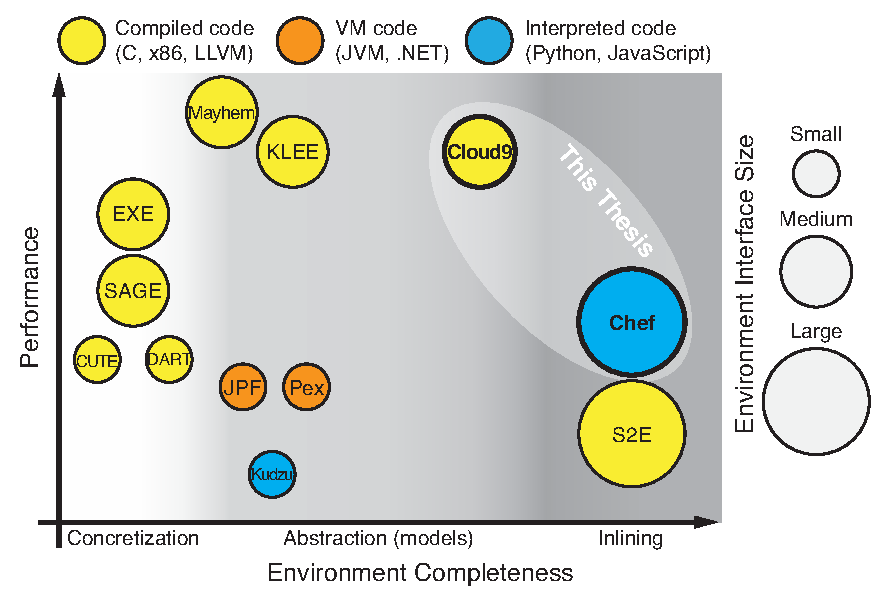
\includegraphics[width=0.8\textwidth]{relatedwork/figures/relwork-positioning}
  \caption{Qualitative comparison of most important symbolic execution engines with respect to the environment problem. X axis indicates completeness of symbolic environment, ranging from no symbolic support (concretization) to full environment inlining.  Y axis indicates relative performance of engines in terms of paths throughput, as deduced from each engine's evaluation numbers.}
  \label{fig:relwork:positioning}
\end{figure}

To efficiently handle real-world programs, symbolic execution engines need to minimize the time spent in the environment, while ensuring correct behavior in the program.
%
Existing approaches roughly fall into three categories, according to the degree of completeness in handling symbolic data going to the environment: (1) concretizing the calls to the environment (no symbolic support at all), (2) abstracting away the environment complexity through models, and (3) ``inlining'' the environment with the program.

Figure~\ref{fig:relwork:positioning} positions the existing work with respect to this classification, while qualitatively indicating the size of the environment interface targeted by the engine and the relative performance attained by each engine in its class.
%
There are several patterns emerging from this classification.

First, the less complete the environment support, the higher the engine performance tends to be.
%
A simpler environment creates fewer execution paths and leads to simpler symbolic expressions in the program state.  In turn, the path throughput in the target program increases.
%
This effect is most visible in symbolic execution engines that resort to concretization or employ simple models, such as EXE~\cite{exe}, Mayhem~\cite{mayhem}, or KLEE~\cite{klee}.

Second, the completeness of the environment tends to be proportional to the complexity of the environment interface of the programs targeted.
%
For example, S2E~\cite{s2eSystem} executes device drivers together with the kernel, as modeling the latter would be too expensive.

Third, the engine performance at a given environment completeness level (a vertical in Figure~\ref{fig:relwork:positioning}) depends on the targeted language and the constraint solver performance.
%
Engines targeting compiled code (e.g., KLEE~\cite{klee} or SAGE~\cite{godefroid:fuzz}) are typically faster than engines targeting high-level code (e.g., Kudzu~\cite{saxena-kudzu} or Java PathFinder~\cite{jpf-symbex}).
%
Similarly, newer engines that rely on faster solvers (e.g., EXE~\cite{exe}, SAGE~\cite{godefroid:fuzz}, or KLEE~\cite{klee}) fare better than the early engines (e.g., DART~\cite{dart} or CUTE~\cite{cute}).

Finally, Figure~\ref{fig:relwork:positioning} shows that symbolic execution engines make a \emph{tradeoff} between the completeness of their environment and the performance they are willing to sacrifice.
%
From this perspective, our contributions, embodied in the \chef and \cnine symbolic execution engines, advance the state of the art by improving this tradeoff.
%
Cloud9 retains the performance of model-based environment handling, while providing an accurate operating system model that comes closer in completeness to an inlined approach.
%
Chef benefits from the completeness of inlining the environment---the language interpreter---with the interpreted program, while significantly improving performance over na\"{\i}ve symbolic execution.

In the rest of this section, we discuss in more detail each of the three environment approaches.
%
We use the program in Figure~\ref{fig:relwork:example} as a running example to illustrate the tradeoffs made by each approach.

\begin{figure}
  \centering
  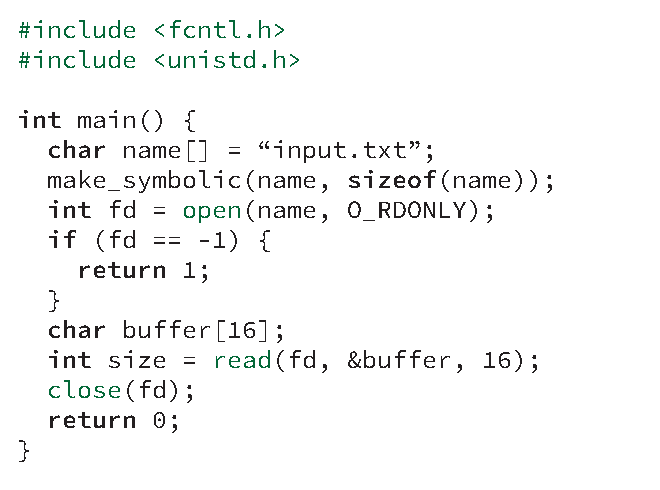
\includegraphics[width=0.6\textwidth]{relatedwork/figures/environment-example}
  \caption{Example of C program using the POSIX operating system interface to open and read a file.}
  \label{fig:relwork:example}
\end{figure}

\subsection{Over-approximation (Concretization)}

A simple approach to simplifying the environment execution is to concretize the values that cross the program boundary~\cite{dart,godefroid:fuzz,klee,exe}.
%
For instance, when a symbolic value $\mu$ is passed as a parameter to an external function, the symbolic execution engine replaces the symbolic expression with a concrete example $m$.  This causes the execution to proceed linearly inside the environment.

For simple programs with limited interactions with their environment, this approach is sufficient.  However, for programs with stronger connections to the environment---e.g., maintaining open file descriptors---concretization may cause missed feasible paths and inconsistencies.

Consider the example of an environment call with symbolic arguments.  Concretization affects both the return value and the input arguments.
%
First, the return value is always concrete, which may lead the symbolic execution engine to miss value-dependent paths in the program, such as error handling.
%
Second, in order to maintain soundness, concretization introduces constraints in the path condition that bind the symbolic arguments to concrete examples (in our case, $pc_{new} := pc_{old} \wedge (\mu = m)$).  This, too, restricts the possible executions on the paths following the external call.
%
Avoiding the extra conditions might increase the coverage of the target program, at the expense of potentially introducing false executions.

A concrete environment may also introduce inconsistencies if it is shared among all execution paths~\cite{klee}.
%
This is commonly the case with non-concolic (``purely-symbolic'') execution, when the symbolic execution engine maintains all execution states as data structures in its address space.  Calls to the environment would then be passed on to the environment of the engine itself, potentially causing cross-talking between different execution paths.

\subsection{Abstraction (Modeling)}

An alternative approach to simplifying the environment is to replace its concrete implementation with a simpler one---a model---that captures its essential behavior~\cite{klee,mayhem,aeg}.
%
The model is smaller---often by orders of magnitude---than the original implementation, as it drops non-functional requirements, such as performance or fault-tolerance.  For example a key-value store database dependency of a web application could be replaced with a plain dictionary when symbolically executing it.

Symbolic execution engines implement models either by building them into the engine implementation (e.g., symbolic hardware models in S2E~\cite{s2eSystem}), or as guest code running together with the target program (e.g., the file system models in KLEE~\cite{klee}).

Although they are effective at reducing path explosion, models are expensive to write correctly and completely.  As a result, they tend to be employed only for simple or stable environment semantics, or when the model accuracy is less important (e.g., security testing~\cite{aeg}).

Cloud9 takes the modeling approach to the environment problem, when symbolically executing programs interacting with the operating system.  Cloud9 is the first to provide an accurate and efficient model for an operating system interface as complex as POSIX.  Key to our approach is to divide the model code into built-in core primitives and guest code, which helps keep the implementation simple, while covering much of the most common operating system abstractions.

\subsection{Inlining (Whole-system Analysis)}

Concretizing environment calls or writing models is unfeasible when the environment interface is large or maintains a complex state, strongly coupled to the program state.
%
For example, once loaded, a device driver typically can interact with the entire operating system kernel.  Concretizing all kernel calls would drastically reduce the exploration space, while modeling all kernel features would be expensive, especially for kernels with high internal churn, such as Linux.

For these cases, an approach that preserves correctness and completeness is to bundle the environment with the program and execute it symbolically as one target.
%
Full-VM symbolic execution engines provide this approach~\cite{s2e,bitBlaze}.

However, this approach reduces the effectiveness of symbolic execution on the original target program, due to the path explosion in the entire system, which may be orders of magnitude larger than the program.
%
To mitigate the path explosion, S2E introduces execution consistency models, which are principles of converting between symbolic and concrete values when crossing the program boundaries, in order to control the path explosion in the environment.

Chef takes the inlining approach to the environment problem, when symbolically executing programs written in interpreted languages.  Chef is the first system to use a language interpreter as a semantics provider for symbolic execution.


\subsection{Developer Control of Symbolic Environments}

The developer interface to a symbolic execution engine plays an important role in controlling its effectiveness and efficiency.
%
The best known sources of developer inputs are the search selection strategies and the injection of symbolic data in the system.
%
For example, KLEE runs command-line utilities with symbolic arguments defined using a special syntax, in line with the rest of the target arguments.  For instance, \codebit{ls -l --sym-arg 1 3} runs \codebit{ls} with the second argument symbolic, between 1 and 3 characters.  This syntax can be used to define symbolic arguments or symbolic files.

The developer control over the symbolic input was encapsulated in concepts such as parameterized unit tests~\cite{tillmann-puts}, which extend regular unit tests with parameters marked as symbolic inputs during symbolic execution.
%
Similarly, QuickCheck~\cite{quickcheck} allows writing input specifications in Haskell, which are used to instantiate inputs during random testing.

However, systems software is influenced by many other external factors, such as environment variables, system call failures, thread schedules, signal dispatch timing, and so on.
%
To address this problem, Cloud9's symbolic test interface gives extensive control over the behavior of its operating system model, such as per-file descriptor symbolic fault injection or per-socket symbolic control flow.

%%% Local Variables: 
%%% mode: latex
%%% eval: (visual-line-mode)
%%% fill-column: 1000000
%%% TeX-master: "main"
%%% End:
